%-----------------------------------------------------------------------------
%
%               Template for sigplanconf LaTeX Class
%
% Name:         sigplanconf-template.tex
%
% Purpose:      A template for sigplanconf.cls, which is a LaTeX 2e class
%               file for SIGPLAN conference proceedings.
%
% Guide:        Refer to "Author's Guide to the ACM SIGPLAN Class,"
%               sigplanconf-guide.pdf
%
% Author:       Paul C. Anagnostopoulos
%               Windfall Software
%               978 371-2316
%               paul@windfall.com
%
% Created:      15 February 2005
%
%-----------------------------------------------------------------------------


\documentclass[preprint,10pt]{sigplanconf}
% The following \documentclass options may be useful:

% preprint      Remove this option only once the paper is in final form.
% 10pt          To set in 10-point type instead of 9-point.
% 11pt          To set in 11-point type instead of 9-point.
% numbers       To obtain numeric citation style instead of author/year.
\usepackage{enumerate}
\usepackage{fancyvrb}
\usepackage{amsmath}
\usepackage{amssymb}
\usepackage{color}
\usepackage{syntax}
\usepackage[style=math]{k}
%\usepackage[style=math]{k}
%\PassOptionsToPackage{pdftex,usenames,dvipsnames,svgnames,x11names}{xcolor}
\PassOptionsToPackage{pdftex}{hyperref}
\usepackage[style=math]{k}


% Slightli modified original version of \reduce. Altered baseline for more compactness.
% No support for multiline.
\newcommand{\reduceClassic}[2]{\hbox{%
  \begin{tikzpicture}[baseline=(top.south), %(top.base), - default, less compact
                      inner xsep=0pt,
                      inner ysep=.3333ex,
                      minimum width=2em]
    \path
          % Original version. No support for line wrapping.
          node (top) [inner ysep=1ex]{$#1$ \mathstrut}

          % New version. Line wrapping support.
          %node (top) [inner ysep=1ex]{$ \begin{array}{@{}c@{}} #1 \end{array} $ \mathstrut}
          (top.south)
          % Original version. No support for line wrapping.
          node (bottom) [anchor=north, inner ysep=.5ex] {$#2$};

          % New version. Line wrapping support.
          % Adds a little bit of vertical space, but the difference is truly insignificant. All the experiments below failed to remove it.
          %node (bottom) [anchor=north, inner ysep=.5ex] {$ \begin{array}{@{}c@{}} #2 \end{array} $};
          % no extra effect
          % node (bottom) [anchor=north, inner ysep=.5ex] {\vspace{-1em} $ \begin{array}{@{}c@{}} #2 \end{array} $};
          % trying mathstrut - some horizontal re-alignment, but no vertical
          % node (bottom) [anchor=north, inner ysep=.5ex] {$ \begin{array}{@{}c@{}} #2 \end{array} $ \mathstrut};
          % no outer ysep (if no inner - looks bad)
          %node (bottom) [anchor=north, inner ysep=.5ex, outer ysep=0] {$ \begin{array}{@{}c@{}} #2 \end{array} $};
          % \vskip -1em just don't compile no matter where we put it
    \path[draw,thin,solid] let \p1 = (current bounding box.west),
                               \p2 = (current bounding box.east),
                               \p3 = (top.south)
                           in (\x1,\y3) -- (\x2,\y3);
    % Solid arrow (augmenting the solid line).
    \path[fill] (top.south) ++(2pt,0) -- ++(-4pt,0) -- ++(2pt,-1.5pt) -- cycle;
  \end{tikzpicture}%
}}

% Defalut version of \reduce in this document.
%   Support for multi-line LHS and RHS
%   Good compactness. Separators adjusted to be aligned with \reduceClassic
\newcommand{\reduceMulti}[2]{\hbox{%
  \begin{tikzpicture}[baseline=(top.south), %(top.base), - default, less compact
                      inner xsep=0pt,
                      inner ysep=.3333ex,
                      minimum width=2em]
    \path
          % New version. Line wrapping support.
          node (top) [
            %inner ysep=1ex
            inner ysep=0.6ex
          ]{ $ \begin{array}{@{}c@{}}
                #1
               \end{array} $ \mathstrut}
          (top.south)
          % New version. Line wrapping support.
          node (bottom) [
            anchor=north,
            %inner ysep=.5ex
          ] {
            $ \begin{array}{@{}c@{}}
              #2
            \end{array} $};
    \path[draw,thin,solid] let \p1 = (current bounding box.west),
                               \p2 = (current bounding box.east),
                               \p3 = (top.south)
                           in (\x1,\y3) -- (\x2,\y3);
    % Solid arrow (augmenting the solid line).
    \path[fill] (top.south) ++(2pt,0) -- ++(-4pt,0) -- ++(2pt,-1.5pt) -- cycle;
  \end{tikzpicture}%
}}

%Special version of \reduce with modified baseline, for better rendering of multiline
% LHS and RHS
\newcommand{\reduceCompact}[2]{\hbox{%
  \begin{tikzpicture}[baseline=(bottom), %(top.base), - default, less compact
                      inner xsep=0pt,
                      inner ysep=.3333ex,
                      minimum width=2em]
    \path
          node (top) [inner ysep=0.6ex]{$ \begin{array}{@{}c@{}} #1 \end{array} $ \mathstrut}
          (top.south)
          node (bottom) [anchor=north] {$ \begin{array}{@{}c@{}} #2 \end{array} $};
    \path[draw,thin,solid] let \p1 = (current bounding box.west),
                               \p2 = (current bounding box.east),
                               \p3 = (top.south)
                           in (\x1,\y3) -- (\x2,\y3);
    % Solid arrow (augmenting the solid line).
    \path[fill] (top.south) ++(2pt,0) -- ++(-4pt,0) -- ++(2pt,-1.5pt) -- cycle;
  \end{tikzpicture}%
}}

%\renewcommand{\reduce}[2]{\reduceClassic{#1}{#2}}
\renewcommand{\reduce}[2]{\reduceMulti{#1}{#2}}




\lstset{language=Java,captionpos=t,tabsize=3,frame=no,keywordstyle=\color{blue},
        commentstyle=\color{gray},stringstyle=\color{red},
        breaklines=true,showstringspaces=false,emph={label},
        basicstyle=\ttfamily}

% Required in order to make \kall cells inside comments black.
\renewcommand{\kall}[3][black]{\mall{#1}{#2}{#3}}

% Environment "kdefinition" has effect only in poster style, thus in math style may be safely deleted.

%Continuation of a syntax definition on a new line
\newcommand{\syntaxContNewLine}[3][\defSort]{\par\indent\rulebox{%
  $\setlength{\syntaxlength}{\widthof{$\mathrel{::=}$}}%
  \setlength{\syntaxlength}{.5\syntaxlength}%
  \addtolength{\syntaxlength}{\widthof{\syntaxKeyword$#1$}}%
  \hspace{\syntaxlength}%
  \;\;\;\;\;\;\;{#2}$ \ifthenelse{\equal{#3}{}}{}{[#3]}%
  }%\k@markPosition%
}

%Should be put after a syntaxLong.
\newcommand{\syntaxEnd}[3][\defSort]{
  \indent\rulebox{%
  $\setlength{\syntaxlength}{\widthof{$\mathrel{::=}$}}%
  \setlength{\syntaxlength}{.5\syntaxlength}%
  \addtolength{\syntaxlength}{\widthof{\syntaxKeyword$#1$}}%
  \hspace{\syntaxlength}$%
  }%\k@markPosition%
}

\newcommand{\syntaxLong}[3][\defSort]{\rulebox{%
\syntaxKeyword
$
  \begin{array}[t]{@{}l@{}}
  #1 \\
  \mathrel{::=}{#2}
  \end{array}
$ {}%
}%\k@markPosition%
}

% Grigore's idea macro
\newcommand{\idea}[1]{
  \begin{quote}
    \rule{.45\textwidth}{.5pt}\newline
    {\em #1}
    \vspace*{-1ex}\newline \rule{.45\textwidth}{.5pt}
  \end{quote}
}

\newenvironment{ideas}
{ \begin{quote}
    \rule{.45\textwidth}{.5pt}
    \newline
    \begin{em}
} {
    \end{em}
    \vspace*{-1ex}
    \leavevmode
    \newline
    \rule{.45\textwidth}{.5pt}
  \end{quote}
}

%Enforcing black cells
\renewcommand{\kall}[3][white]{\mall{black}{#2}{#3}}
\renewcommand{\kallLarge}[3][white]{\mallLarge{black}{#2}{#3}}
\renewcommand{\kprefix}[3][white]{\mprefix{black}{#2}{#3}}
\renewcommand{\ksuffix}[3][white]{\msuffix{black}{#2}{#3}}
\renewcommand{\kmiddle}[3][white]{\mmiddle{black}{#2}{#3}}

% Settigns required for Chucky's background section
\usepackage{acronym}

\providecommand{\Sec}{}
\renewcommand{\Sec}{Section~}
\newcommand{\Fig}{Figure~}

\newcommand{\cellname}[1]{\textsf{#1}}

\newcommand{\kequation}[2]{\begin{equation*}{\small#2}\end{equation*}}

%Probably a mapsto with spacing
\newcommand{\mapstox}{\small\mathrel{\mapsto}}

%For spacing between cell lines
%\newcommand{\kBR}{\\[0.3em]}

% The following packages can be found on http:\\www.ctan.org
\usepackage{graphicx} % for pdf, bitmapped graphics files
% General
\newcommand{\w}[1]{\ensuremath{\textit{#1}}}
\newcommand{\m}[1]{\ensuremath{\texttt{#1}}}
\newcommand{\s}[1]{\ensuremath{\textsf{#1}}}
\newcommand{\p}[1]{\ensuremath{\left(#1\right)}}
\newcommand{\pl}[1]{\ensuremath{\left\langle#1\right\rangle}}
\newcommand{\OR}{\mbox{ }|\mbox{ }}
\newcommand{\st}{.\mbox{ }}
\newcommand{\finto}{\ensuremath{\stackrel{\mathtt{fin}}{\longrightarrow}}}
\newcommand{\defeq}{\ensuremath{\stackrel{\mathtt{def}}{=}}}
\newcommand{\cond}[1]{\ensuremath{\left\{\begin{array}{ll} #1 \end{array}\right.}}
\newcommand{\lst}[1]{\begin{itemize} {#1} \end{itemize}}
\newcommand{\pby}[1]{\hspace*{\fill}{#1}}
\newcommand{\slide}[2][]{ \begin{frame} \frametitle{#1} {#2} \end{frame} }
\newcommand{\etal}{\textit{et al.}\xspace}
\newcommand{\rolang}{PCCL }
\newcommand{\StarL}{StarL\xspace}

% For references
\newcommand{\fig}[1]{Figure~\ref{#1}}
\newcommand{\lem}[1]{Lemma~\ref{#1}}
\newcommand{\theo}[1]{Theorem~\ref{#1}}
\newcommand{\coro}[1]{Corollary~\ref{#1}}
\newcommand{\defn}[1]{Definition~\ref{#1}}
\newcommand{\rmrk}[1]{Remark~\ref{#1}}
\newcommand{\exam}[1]{Example~\ref{#1}}
\newcommand{\sect}[1]{$\S$~\ref{#1}}
\newcommand{\refsect}[1]{Section~\ref{sect:#1}}
\newcommand{\reffig}[1]{Figure~\ref{fig:#1}}

\definecolor{orange}{rgb}{1,0.5,0}
\definecolor{darkgreen}{rgb}{0.0, 0.5, 0.0}
\newcommand{\marker}[1]{} %{\note{orange}{{#1}}}
\newcommand{\SM}[1]{\note{darkgreen}{SM: {#1}}}
\newcommand{\RG}[1]{\note{orange}{RG: {#1}}}


\makeatletter
\newcommand*{\centerfloat}{%
  \parindent \z@
  \leftskip \z@ \@plus 1fil \@minus \textwidth
  \rightskip\leftskip
  \parfillskip \z@skip}
\makeatother
\newcommand{\cL}{{\cal L}}
\usepackage{mathtools}
\DeclarePairedDelimiter\ceil{\lceil}{\rceil}
\DeclarePairedDelimiter\floor{\lfloor}{\rfloor}
\lstdefinelanguage{myLang}
{
  language     = Java,
  % list of keywords
  morekeywords={
    import,
    if,
    while,
    for,Agent,allwrite,allread,Init,pre,eff,atomic,loc
  },
  sensitive=false, % keywords are not case-sensitive
  morecomment=[l]{//}, % l is for line comment
  morecomment=[s]{/*}{*/}, % s is for start and end delimiter
  morestring=[b]" % defines that strings are enclosed in double quotes
}
\lstdefinestyle{myCustomStyle}{
keywordstyle=\color{blue},
language=myLang,
stepnumber=1,
  numbersep=10pt,
  tabsize=2,
  showspaces=false,
  showstringspaces=false
}
\lstset{basicstyle=\scriptsize,style = myCustomStyle}

\begin{document}

\special{papersize=8.5in,11in}
\setlength{\pdfpageheight}{\paperheight}
\setlength{\pdfpagewidth}{\paperwidth}


% Uncomment the publication rights you want to use.
%\publicationrights{transferred}
%\publicationrights{licensed}     % this is the default
%\publicationrights{author-pays}

\title{PCCL: Physical Coordination and Control Language}
\author{Ritwika Ghosh\qquad Sayan Mitra}
\institute{University of Illinois at Urbana-Champaign\\ \email{rghosh9,mitras@illinois.edu} }


\maketitle
\begin{abstract}
We describe the design of \rolang, a language for writing distributed applications with dynamic behavior. \rolang allows the programmer to write application code, which involves communication between agents using shared memory, and interaction with physical environment using time varying system variables, in a clean and precondition-effect style representation. \rolang also serves as a high level language for the StarL robotic 	 framework. 
We provide an executable formal semantics for \rolang using the $\mathbb{K}$ semantic framework. We use the notion of a parametrized semantics, where the dynamics of the system is governed by an external model. We also provide a time model and discuss communication through shared memory. We then use this \rolang to write various distributed applications and explore their behavior in the executable semantics implemented in $\mathbb{K}$.
\end{abstract}

%\input{terms.tex}
\section{Introduction}
Distributed applications are all pervasive, and have been studied at great depth. Development of distributed applications with physical control components have gained great importance in recent history due to the ever increasing automation in everyday life. These applications can run on platforms which interact with the physical environment (UAVs, self-driven cars, etc.). Development of such applications usually requires expertise of the language in which the applications are written, and experience with the hardware platform on which it will be deployed.  Managing and experimenting with these platforms is usually a time consuming and non trivial task, as most such systems are based on design choices specific to developers abd not standardized.
Deployment and testing of a new algorithm might take a long time for even experienced programmer.  If one wanted to test an existing application different dynamics models, or a new platform, or heterogeneous agents, it could jeopardize time sensitive deployment programs.  Considerably less effort is needed to perform this type of task with desktop (or mobile) applications. The lack of an accepted standard, and abstractions for specific applications makes experiments are costly to repeat and verify. 

In this paper, we present \rolang: a language which enables users to start developing and understanding applications which interact with the physical environment. The user writes code for a single agent, which can be deployed on a multiple agents to perform a distributed task, such as leader election . \rolang provides a clean precondition-effect style of programming, similar to the representation of Hybrid Input-Output Automata as in~\cite{lynch1996hybrid}. HIOA is a mathematical framework for precisely describing
systems that have both discrete and continuous behaviors. The precondition-effect block constitute \emph{events}, which correspond to discrete steps in the HIOA. Control variables change when the external functions are called, corresponding to the continuous trajectory of the HIOA, and this take non-zero time to occur. We introduce a time model in \refsect{time} which guards against zeno behavior of the applications.  

 We designed the semantics of this language, driven by one simple idea. The effect of the interaction with the physical environment is seen only on "control" variables, or variables which are controlled outside the environment. Provided controllers to determine the values of these variables when looked up, the semantics of this language can be specified independently, considering these controllers as external functions which return  values for these variables. We provide several abstractions to the user for communication and physical control. The major design details are captured by the semantics we present in this paper, while the external functions can be implemented by the user if they want to do so. In applications written in \rolang, agents communicate using shared variables. Shared variables in practice are implemented through message passing on hardware platforms. In this paper, we present a semantics which has an eventual consistency, but our design is modular enough to implement different consistency models. In our semantics, the external functions which control interaction with the physical environment are \emph{parameters} provided to the semantics. Several other application specific features can also be provided as external functions, such as communication restrictions based on geographical proximity. We assume that all agents can communicate with all other agents. In \refsect{future}, we discuss our planned implementation of a publish-subscribe model of communication among agents. 

We use the \K semantic framework to write the semantics of this language, as it can be used to generate an executable semantics which lets us run applications and generate execution traces. We talk about \K in \refsect{k}. We implemented several distributed applications using this language, and we discuss two of them in this paper.The executable semantics generated by the \K framework can be used to run applications written in this language.\footnote{https://github.com/ritwika314/PCCL} 
\subsection{Related Work}
\label{sect:rel}
In this work, we have presented the formal semantics of a  language for distributed agent coordination and control. The main focus of this work was on developing a formal model for asynchronous concurrent applications where communication occurs through shared memory. \cite{P} is a language for asynchronous event-driven programming, which allows the programmer to specify the system as a collection of interacting state machines, which communicate with each other using events as opposed to shared memory updates as in \rolang. In an actual implementation (like StarL), agents do respond to message events, which could in principle be modeled in P. Our work provides  a framework that allows a relatively novice user to write pseudocode without being concerned with implementation details.
There are languages such as Esterel \cite{esterel} , Lustre \cite{lustre} and Signal\cite{signal}. As in our model of time evolution, these languages also follow a model where time
advances in steps. However, since we express our semantics in the \K framework, we can explore various interleaving semantics. In these languages, given
a state and an input at the current time step, there is a unique possible
state at the next time step. 
The synchronous model has the advantage that every event
sent to machine is handled in the next clock tick, and is widely
used in hardware and embedded systems. However, in an OS or a
distributed system, it is impossible to have all the components of
the system clocked using a global clock, and hence asynchronous
models are used for these systems, which gives a language like P an advantage over \rolang. In such models events are
queued, and hence can be delayed arbitrarily before being handled. Theoretically, we can also model delays like this by enforcing application of specific rewrite rules repeatedly, but that would limit the generality of the semantics. 

\section{Overview of Language and System}
\label{sect:Overview}
In this section, we give an overview of the whole system architecture within which \rolang programs executed and then discuss key language features with an example.

We call an entity executing a \rolang program an {\em agent\/} or a {\em process.\/}
The hardware abstraction on which \rolang programs executes includes (a) a controller, (b) shared memory, in addition to the usual (c) local memory and processing unit of the agent.  
%
The controller receives lists of way-points and obstacles from the agent's program, drives the actuators (e.g. motors) to reach the way-points while avoiding the obstacles using sensors (e.g. GPS), and updates certain flags to indicate its status to the program.
%
The shared memory abstraction provides single-writer and multi-writer distributed shared variables using which an agent's program can communicate with another agent's program. 

A \rolang program interacts with 
\begin{figure}[t!]
	\centering
	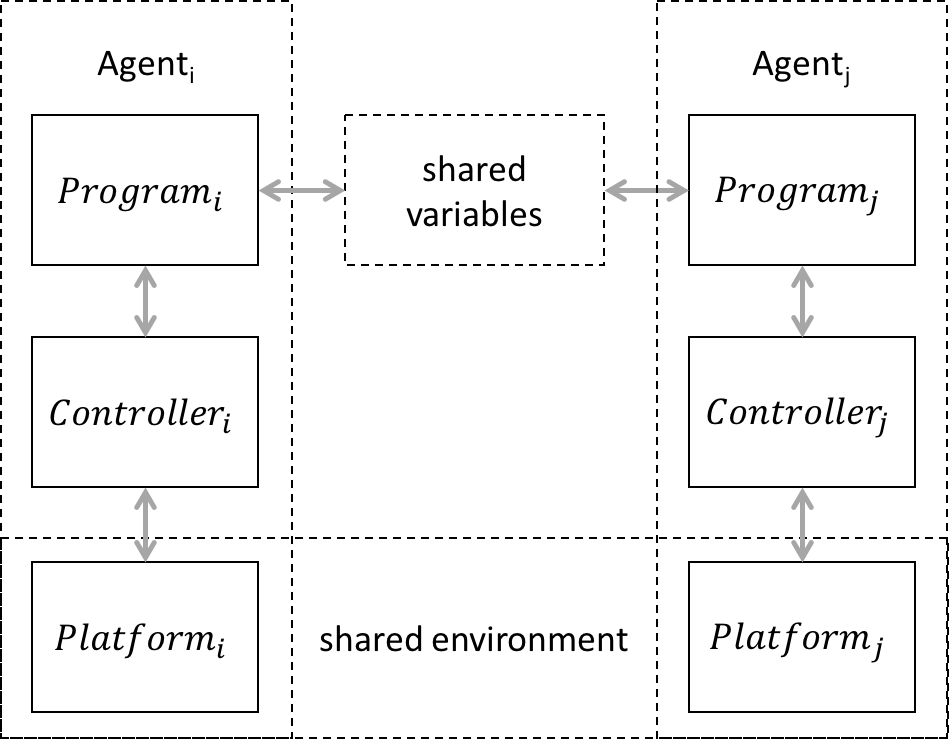
\includegraphics[scale=0.4]{figs/arch.png}
	\caption{\small Architecture of distributed system. Agent programs interact through shared variables. Each agent program also sets waypoints for its own controller which control the physical motion of the agent's platform. The agent platforms inhabit a shared physical environment, and therefore, also interact physically.}
\end{figure}

\rolang allows users to write applications that will run on a distributed system of agents. The user writes a program as though for a single agent, and all agents execute the same code. A \rolang program is a collection of \emph{declarations} and \emph{events}. Shared variables are used for communication between agents. They are declared in an \verb|MW| block. \verb|MW| stands for \emph{multi-writer}, implying that all agents can read from, and write to the variables declared in this block. We provide another type of shared variables called \emph{shared single-writer} variables, which all agents can read from, but only one agent can write to. These variables are parameterized by the \verb|agent index|, an integer which is a unique identifier for each agent in the system, and they are declared in the \verb|SW| block. Local variables are declared in \verb|Loc|al declaration blocks.  \newline

As mentioned earlier, \rolang uses a \emph{precondition-effect} style of programming. These precondition and effect statements form events. Each application consists of a special \verb|Init| event, and an \verb|EventBlock|. The \verb|Init| event occurs at the beginning when the application starts executing, and it contains all statements which need to be executed only once; for instance, initializing a shared array. After the \verb|Init| event is executed, the \verb|EventBlock| starts executing. It contains a list of events that define the behavior of the application. The preconditions of each of the events inside the \verb|EventBlock| are evaluated in order of appearance, and the effect is executed if the precondition becomes true. The \verb|EventBlock| can be seen as a (potentially) infinite while-loop. 

We also provide an abstraction to manage the physical control of the agents, called \verb|doReach|, which takes as input a \emph{target} to reach, and a list of (predetermined) \emph{obstacles} which need to be avoided. We do not need to specify the format of the obstacles, as different implementations of this \verb|doReach| can have different specifications, but the target in general has the same type as the time varying variables of the system. \verb|doReach| communicates with the program using two flags, \emph{doReach_done}, and \emph{doReach_fail}. If the target is reached, the \emph{doReach_done} is set to true, and the \emph{doReach_fail} is set to true when the agent does not seem to have reached the target.

The next section presents the formal syntax, and an example to illustrate the structure of a general application. 

\subsection{Syntax}
\label{sect:syntax}
This section describes the formal syntax of \rolang. We first provide the major features of the formal syntax which describe program structure, event structure, and statement structure. 
\begin{figure}[ht!]
\footnotesize
\begin{center}
\noindent\begin{minipage}{.45\textwidth}
\begin{grammar}
<Pgm> :: <VarDecls><InitBlock><EventBlock>

<VarDecls> :: <MwDecls><SwDecls><LocDecls>

<MwDecls> :: "MW :" <Decls>

<SwDecls> :: "SW :" <Decls>

<LocDecls> :: "Loc :" <Decls>

<Decls> :: <Decl> <Decls> \\
         | <Empty>

<Decl> :: <EnumDecl> ";" \\
         | <ArrayDecl> ";" \\
         | <Type> <Var> ";"\\
         | <Type> <Var> "=" <Expr>
 
<InitBlock> :: "Init :" <Stmts>
\end{grammar}
\end{minipage}\hfill
\noindent\begin{minipage}{.45\textwidth}
\begin{grammar}
<EventBlock> :: "EventBlock:" <Events>

<Events> :: <Event><Events> | <Event>

<Event> :: <EventName> "(" <Expr> ")" "Pre" "(" <Expr>")" ";" "Eff :" <Stmts> 

<Stmts> :: <Stmt><Stmts> \\
		| <Empty>

<Stmt> :: <Assignment> \\
		| <If-Then-Else> \\
        | <Loop>\\
        | <Atomic>
		| <FunctionCall>
        
<Atomic> :: "Atomic :" Stmts
\end{grammar}
\end{minipage}
\end{center}
\caption{Language Syntax Features}
\end{figure}
As mentioned in the overview, each program consists of three major parts, with variable declarations, an initialization block and an event block. Aside from usual data types and arrays, we provide support for declaring enumerated types, as it is easy to use them as "stages" in applications.\footnote{https://github.com/ritwika314/RoLang/StarL/HLL/Examples/LeaderElect}

Events, as mentioned earlier are specified by precondition-effect blocks, where the precondition is a boolean expression, and effect blocks contain statements, which can be assignment statements, \verb|if-then-else| statements, \verb|Atomic| statements, function calls, or loops. We omit the productions for the more obvious syntactic elements like expressions, assignment statements, loops, etc.\footnote{https://github.com/ritwika314/RoLang/StarL/HLL/Semantics/agent-syntax.k}
\section{Preliminaries}
\label{sect:Prelim}

\subsection{The \textbf{K} Framework}
\K~\cite{rosu-serbanuta-2013-k} is a rewrite-based executable framework for defining language semantics.
Given a syntax and a semantics of a language, \K generates a parser, an interpreter, as well as formal analysis tools such as model checkers and deductive program verifiers at no additional cost.
\K also provides several formal analysis tools, which will enable us to perform formal reasoning about the language we have defined using this framework. 

This helps both in terms of applicability of the semantics and in terms of engineering the semantics itself; for instance, the state-space exploration capability helps the language designer cover all the non-deterministic behaviors of certain language constructs or combinations of them in the language definition.

We briefly describe \K here. In \K, a language syntax is defined using conventional Backus-Naur Form (BNF).
A language semantics is given as a transitions system, specifically a set of reduction rules over configurations.
A configuration is an algebraic representation of the program code and state.
Intuitively, it is a tuple whose elements (i.e. cells) are labeled and possibly nested. 
Each cell represents a semantic component such as store, environment and thread that is used in the semantics.
A special cell, named \s{k}, contains a list of computation to be executed.
A computation is a program fragment, while the original program is flattened into a sequence of computations or programming tasks.
A rule describes a one-step transition between configurations.
Rules are modular; they mention only relevant cells needed in each rule.
The cells are represented with angle brackets notation.
The horizontal line represents a reduction (i.e. a transition relation).
A cell with no horizontal line means that it is read but not changed by the rule.

To model the behaviors and interactions between agents, an appealing aspect of \K is its inherent support for non-determinism.
As \K is based on rewriting logic \cite{meseguer2007rewriting}, one can easily define, execute, and reason about non-deterministic specifications in \K. 
\K can capture non-deterministic features both related to concurrency and to the order of evaluation. 

\subsection{The \StarL robotics framework}
We are developing \rolang to interface with the Stabilizing Robotics Language (\StarL). 
\StarL is primarily in Java, and it provides language constructs for coordination and control
across robots.Two key features of \StarL are a distributed shared memory (DSM) primitive
for coordination and a reach-avoid primitive for control. DSM allows a
program to declare program variables that are shared across multiple robots
. This enables programs running on different
robots to communicate by writing-to and reading from the shared variable.

All the program threads implementing the application, the message channels,
as well as the physical environment of the application (robot chassis, obstacles)
are modeled as hybrid automata, and the overall system is described
by a giant composition of these automata. 
\section[h]{Formal Semantics}
\label{sect:semantics}

In this section we describe the formal semantics of key language elements. 
The system consists of \textbf{N} agents $A_1$, ..., $A_N$. The state of the overall system advances by two types of transitions: 
(a) {\em program transitions\/} correspond to agent program events updating agent variables and possibly setting waypoints for the agent's controllers. Program transitions take zero logical time.
(b) {\em environment transitions\/} 
correspond to the physical environment of the agent evolving over an interval of time. During this period, the agent platforms may be moved by their controllers, messages implementing the distributed shared memory abstraction are propagated. 
Environment transitions  are external to \rolang, and therefore, in providing an executable semantics these transitions have to be implemented by external function(s).
%
Thus, a given \rolang program may be executed with different  external functions, to obtain different executions.
% resume here.
%In doing so we use a parametrized formal semantics, where the parameters govern the intervals at which the system is observed(\refsect{exec}) and how the system evolves with respect to time(\refsect{dynamics}). Essentially, we specify the semantics of the language, provided there is a procedure to compute the physical control component of a system. 
%
For instance, in the race application described in \refsect{Eg}, we parameterize the language semantics with the procedure for computing the positions of the robots at a given time. The event block is like the discrete step of a hybrid automaton, and the dynamic behavior is the continuous trajectory\cite{hioa}. The discrete part of the system corresponds to the programs, which interact with the physical environment using the \s{doReach} abstraction. The programs communicate with each other using shared variables.

We explain this further in the following sections, starting with a description of the system state. We then describe the major features of the language semantics, including the time model and the dynamics model, which parametrize the semantics. 

\sayan{resuming here}

 
 


In \refsect{syntax}, we described the structure of applications written in this language; each application is written in terms of events. We say that an event has occurred if its precondition was evaluated as true, and the corresponding effect was executed. Once an event has occurred, the program control goes back to the top of the event block. The event block (\s{eventBlock}) is said to be executed when any event in the event block occurs once. Given an agent running an application, its event block can be executed repeatedly while the application continues to run. Communication between agents takes place through shared memory updates. Shared memory updates require mutual exclusion, which is implemented by a locking mechanism. We describe the \verb|atomic| construct, which is used for mutual exclusion, in \refsect{locking}.


\subsection[h]{Configuration}
The configuration, or state, holds program variables, objects, and the execution context. We omit implementation minutiae, and only show relevant features. In the configuration, an agent is represented by an \s{agent} cell. Recall that a cell is a configuration unit, which is denoted by $\langle \mbox{cell-type} \rangle_{\mbox{cell-name}}$. For instance, a cell maintaining the \s{position} of an agent, which has type \verb|ItemPosition| will be represented as $\langle {\verb|ItemPosition|} \rangle_{\s{position}}$. Cells can also be composite cells, or containers of other cells. They will just be denoted by $\langle\mbox{cell-contents}\rangle_{\mbox{cell-name}}$.  

Each agent is represented by a composite cell, because the code is executed at agent level, and requires agent-specific information. An \s{agent} is identified by a unique identifier \s{id} (which is an integer). Its configuration contains the following cells. 
\begin{itemize}
 \item  \s{k} : Contains an agent's own application code. Each line in this cell is rewritten (possibly to empty) as the semantics is executed.
 \item \s{id} : Contains the agent's unique integer identifier. 
 \item \s{memory} : Contains a map from variables to addresses. 
 \item  \s{position} : The current position of the agent. Note that we only include the position cell in the current semantics because the applications we intend to write are in the domain of robotics. We can create cells to time-varying attributes of the agents as required.  
 \item  \s{counter} : The \s{counter} cell of each agent in the configuration maintains the number of times the event block of that agent has executed.
 \item \s{lockState} : Denotes whether or not the agent holds the requested lock. We discuss locking in \refsect{locking}. 
\end{itemize}
\begin{figure*}[ht]
\large
\centerfloat
  %
  \renewcommand{\dotCt}[1]{\scriptstyle\textit{#1}}
  \newcommand{\rid}{\scriptstyle\textit{ID}_{\sf robot}}
  \newcommand{\env}{\scriptstyle\textit{Var} \;\mapsto\; \textit{Address}}
  \newcommand{\store}{\scriptstyle\textit{Address} \;\mapsto\; \textit{Value}}
  %
$
\kall{system}{
  \begin{array}{@{}c@{}}
     \kall{k}{\dotCt{K}} \mathrel{}
      \kall{id}{\dotCt{Int}}\mathrel{}
      \kall{memory}{\dotCt{.Map}} \mathrel{}
      \kall{position}{\dotCt{ItemPosition}} \mathrel{}
      \kall{counter}{\dotCt{Int}} \mathrel{}
      \kall{lockState}{\terminal{idle}}
  \\ \mathrel{}
  \end{array}
}
$
  %
\caption{Agent Configuration}
\label{fig:agentconfig}
\end{figure*}

\normalsize

 Each agent's \s{memory} cell is a map from \emph{all} variables(of type \s{Id}, short for string identifier), to addresses(of type \s{Int}). Both global and local variables are included in this \s{memory}. This amounts to maintaining local copies of global variables, which are consistent across agents.  
 
The top level cell is called the \s{system cell}, which represents the distributed agent system. This cell contains the following cells:
\begin{itemize}
\item \s{agents} : This is a container cell for \s{agent} cells. It can contain as many such cells as the number of agents running the application, denoted by multiplicity "*". 
\item \s{gMemory} : This is the global memory, contains a map from all shared variables to addresses in the memory . 
\item \s{MMap} : Each variable of the application has an address in memory; we will presently discuss the scope of said memory. \s{MMap} stands for memory map, which is a map from addresses in the memory to actual values corresponding to the variables. 
\item  \s{time} : This is cell for maintaining time elapsed. 
\item \s{counterMap} : This cell maintains the map of agent \s{ids} to their \emph{counter} (\refsect{exec}) values. We explain what that refers to, in the next paragraph. 
\item  \s{lockQueue}: This cell is used to maintain the order in which the lock requests have been made.
\item \s{transitionState} : This cell stores whether the system is currently demonstrating dynamic behavior or not.  
\end{itemize}
\begin{figure*}[ht]
\large
\centerfloat
  %
  \renewcommand{\dotCt}[1]{\scriptstyle\textit{#1}}
  \newcommand{\rid}{\scriptstyle\textit{ID}_{\sf robot}}
  \newcommand{\env}{\scriptstyle\textit{Var} \;\mapsto\; \textit{Address}}
  \newcommand{\store}{\scriptstyle\textit{Address} \;\mapsto\; \textit{Value}}
  %
$
\kall{system}{
  \begin{array}{@{}c@{}}
  \kall{agents}{
  	agent*
  } \mathrel{}
  \\ \mathrel{}
  \kall{gMemory}{\dotCt{.Map}}\mathrel{}
  \kall{MMap}{\dotCt{.Map}} \mathrel{}\\ 
  \mathrel{} \kall{time}{\dotCt{Int}} \mathrel{}
   \kall{counterMap}{\dotCt{.Map}} \mathrel{}
  \kall{lockQueue}{\dotCt{.List}} \mathrel{} \\
  \kall{transitionState}{\terminal{discrete}}\mathrel{}
  \\ \mathrel{}
  \end{array}
}
$
  %
\caption{System configuration.}
\label{fig:highlevelconfig}
\end{figure*}

\normalsize


\subsection[h]{Local Variable Declaration}
We first provide the semantic rules for processing variable declarations, as an introduction to reading the semantic rules in \K. When a local variable declaration is encountered while an agent's code is being processed, an entry is created in the \s{memory} cell, which maps the variable to the next available address in the \s{MMap}. A corresponding entry is created in the \s{MMap}, which maps the aforementioned address to an \s{undefined} value of the declaration type if the declaration is uninitialized. It maps to the value the variable was assigned otherwise. We now define the rule for local variable assignment.
\paragraph{Variable declaration rule: } The \s{k} cell of an agent holds the code being interpreted. Suppose we encounter a local variable declaration \s{T X;} where \s{T} is the type, and \s{X} is the name of the variable.  We use the ellipses to represent the fact that (possibly empty) contents of the cell after the element being rewritten do not matter. The variable declaration rule first rewrites the line of code to empty($\dotCt{}$). At the same time, it creates an entry in the \s{memory} cell which maps \verb|X| to \s{L}, where \s{L} is the next available address in the \s{MMap}. Creating an entry in the map is the same as rewriting an empty element to the entry at the end of the map, hence the rewrite rule has the form $\reduce{\dotCt{}}{{M}}$, where $M$ is the entry being created.

We omit the details of how we determine $L$, as it is not relevant. The rule also creates an entry in \s{MMap} with \s{L} corresponding to \s{undefined(T)} (undefined value of type \s{T}).  

\begin{figure*}[ht]
\krule[variable declaration]{
\kmiddle{agent}{
\kprefix{k}{
 \reduce{{\variable[type]T \variable[ID]X;}}{{}{\dotCt{}}} }
 \ksuffix{memory}{ \reduce{{\dotCt{}}}{{}{X \mapsto L}}}
}
\ksuffix{MMap}{
 \reduce{\dotCt{}}{{}{L\mapsto undefined(T)}
}}
}
{}{}{}{}
\krule[variable declaration with assignment]{
\kmiddle{agent}{
\kprefix{k}{
 \reduce{{\variable[type]T \variable[ID]X = V;}}{{}{\dotCt{}}} }
 \ksuffix{memory}{ \reduce{{\dotCt{}}}{{}{X \mapsto L}}}
}
\ksuffix{MMap}{
 \reduce{\dotCt{}}{{}{L\mapsto V}
}}
}
{}{}{}{}
\end{figure*}

It should be mentioned that we assume unbounded memory for simplifying the semantics specification.  

\subsection[h]{Time Advance Semantics}
\label{sect:exec}


While designing the current semantics of this language we assume that we are able to maintain a global clock (the \s{time} cell). The dynamic behavior of each agent in the system is time varying. Since global time is a part of the system configuration or state, we need to supply rewrite rules for advancing time.

 Recall that the event block describes the discrete behavior of each agent. We can say that event block execution takes zero logical time. An event block can execute numerous times between time rewrites. We now define the time model for this semantics. The time model $\tau$ is defined as a tuple $\tau = (\delta, n_0)$ where 
 \begin{itemize}
 \item $\delta$ : is the global time increment. 
 \item $n_0$ : is the number of times that the event block of each agent must execute before global time is advanced. We use the \s{counter} and \s{counterMap} cells in the configuration for bookkeeping about this parameter. 
 \end{itemize}
We can now provide the rules of time progression in our semantics, given a time model $\tau = (\delta,n_0)$. 

\paragraph{Counter Advance Transition:}
We first discuss how to increment the \s{counter} of an agent when it executes an event block once. To ensure that, as soon as the precondition of the event evaluates to true, the rest of the event block should be rewritten to empty. That means, given an event block \s{pre(C); eff : S Es} where \s{C} is a condition evaluating to true, \s{S} is the list of statements in the effect of that event, \s{Es} is the list of events following that; this event block rewrites to \s{S}. If \s{C} evaluates to false, this block rewrites to \s{Es}. We skip the details of the rewrite rules involved in this process. 
\s{endEventBlock} is a terminal that we introduce (using a rewrite rule) at the end of the event block. If while executing the semantics, an \s{endEventBlock} is encountered in the \s{k} cell, it should imply that an event has occurred, the \s{counter} should be incremented and  the event block should start executing from the top again.
 
 Consider an agent with \s{id} $i$. If an \s{endEventBlock} is encountered in its \s{k} cell, there is nothing more to do in the current execution. Given further, that the \s{count} cell value of the agent is $N$, the \s{k} cell is rewritten to empty. The \s{counter} cell is rewritten to $N+1$, and the corresponding value of its counter in the \s{counterMap} cell is also rewritten to $N+1$. This transition is enabled only as long as $N$ is less than $n_0$. This ensures that each agent executes its event block exactly $n_0$ times before the time increments. 
\vspace{-1mm}

\begin{figure*}[ht]
\krule[counter advance transition]{
\kall{agent}{
\begin{array}{@{}c@{}}
\kall{k}{
 \reduce{\terminal{endEventBlock}}{{\dotCt{}}}
}
\kall{id}{\variable[Int]i}
\kall{counter}{ \reduce{\variable[Int]{N}}{{{{\variable[Int]{N}}
  \mathrel{+_{\scriptstyle\it Int}}
  {{}\variable[Int]1}}}}}
\end{array}
}
\begin{array}{@{}c@{}}
\kmiddle{counterMap}{ \reduce{\variable[Int]{i}\mapsto N}{{{{{\variable[Int]{i}\mapsto \variable[Int]{N}+_{Int} 1}}}}}}
  \end{array}
}
{
  {{\variable[Int]{N}}
  \mathrel{<_{\scriptstyle\it Int}}
  {{}\variable[Int]n_0}}
}{}{}{}
\end{figure*}

Note that when the \s{endEventBlock} is encountered, we rewrite the entire \s{k} cell to empty. How does the next iteration of the event block start then? We maintain a copy of the original application code in the state information, which is copied into the \s{k} cell at the beginning of every iteration of the event block. We have not shown this (along with other implementation details) in the interest of clarity of expression. 
\paragraph{Time Advance Transition:}
Suppose that the \s{counterMap} cell, which maintains a map of ids to counter values of all agents, is $CM$. \s{findMax} and \s{findMin} are functions for computing the maximum and minimum in the range of a map respectively. If both the minimum and maximum values are equal, then all values in the range of the map are equal.  The \s{time advance} transition says that, given that the current global time is $T$, if all the counter values in $CM$ are equal to $n_0$, the global time is rewritten to $T+\delta$. The \s{transitionState} is set to \verb|dynamic| from \verb|discrete|. We do not show the rest of the configuration items because they do not appear in the condition or change with the time progression rule. 
\begin{figure*}[ht]

\end{figure*}
. 
It is worth mentioning that while we designed the time progression such that the event block executes exactly $n_0$ number of times for each agent, we can easily change the design to accommodate different values for different agents. To do that, we modify the time model by adding another parameter $\rho$ to it. $\rho$ is a map from agent \s{ids} to integers. Instead of incrementing the counter by one every time an event occurs, agent with it $i$ increments its counter by $\rho[i]$. The number of times its event block executes is then $\floor{\frac{n_0}{\rho[i]}}$.


\section[h]{Locking}
\label{sect:locking}
We provide global locks to implement mutual exclusion for the atomic construct. 
	These locks have two major properties:
    \begin{itemize}
\item At any time, at most one agent can hold a lock. 
\item A agent needs to request a lock at most once before being eventually granted the lock. 
\end{itemize}
The first property ensures mutual exclusion and the second ensures that high frequency agents do not monopolize the lock. 
While defining the semantics it is easier for us to present the rules in terms of a single global lock on all multi-writer shared variables. This means that whenever an agent requests a lock it obtains a lock on all shared variables declared in the \verb|MW| block. Each agent has a cell called \s{lockState}, which is set to \s{idle} if the agent is not requesting or holding the lock, \s{request} if the agent has requested the lock but not been granted it yet, and \s{lock} if the agent is currently holding the lock. We maintain the lock queue or the order in which requests to the lock were made by agents, in the cell \s{lockQueue}. 

When an agent requests a lock, its \s{id} is added at the end of the \s{lockQueue} An agent which has requested a lock, is granted it if it is the first in the lock queue. Once an agent has requested a lock, its \s{lockState} is updated to \s{request}. An agent is not allowed to add itself to the \s{lockQueue} unless its \s{lockState} is \s{idle}. When the agent is at the beginning of the \s{lockQueue} and its \s{lockState} is \s{request}, then it can execute its atomic block. Once it has done so, it updates its \s{lockState} to \s{idle} again, and removes itself from the \s{lockQueue}. 

An agent is in the process of executing the effect of an event whose precondition evaluated to true, when it might need to request a lock. It is however, not allowed to execute the next line of code until it is granted the lock and can proceed. We force the \s{counter} to be incremented every time the agent checks its position in the \s{lockQueue}. The reason for this is to capture behavior where the lock may not be granted immediately. From our discussion in the previous section, the event block execution takes zero logical time. If the counters were not incremented while the agents were requesting a lock, all locks would be granted before \s{time} was incremented from the current value. This would then imply that all locks are granted while zero logical time passed, which is unrealistic behavior. We provide the rewrite rules governing locking below, again, given a time model $\tau = (\delta,n_0)$. 

\paragraph{Lock Request Transition:} The \s{lock request} transition is enabled when an agent with \s{id} \s{i}, encounters an atomic block containing statements \s{Ss}, when its \s{lockstate} is \s{idle}. Then, the agent adds a terminal \s{atomicEnd} just after the atomic block, to ensure that the agent releases the lock after executing it. At the same time, the agent adds itself to the end of the lock queue. The ellipses represent the fact that the lock queue may or may not be empty, it doesn't affect the application of the current rule. Again, we omit showing the irrelevant cells in this rule. 
\begin{center}
\begin{figure}
\label{fig:lock1}
\krule[lock request transition]{
\kprefix{agent}{
\begin{array}{@{}c@{}}
\kprefix{k}{\terminal{atomic :}\variable[Statement]Ss
 \reduce{\dotCt{}}{{\terminal{atomicEnd}}}
}
\kall{id}{\variable[Int]{i}}
\kall{lockState}{
 \reduce{\constant[\#Type]{idle}}{\constant[\#Type]{request}}
}

\end{array}
}
\ksuffix{lockQueue}{
{
 \reduce{\dotCt{}}{{\variable[Int]{i}}}
}}
}{}{}{}{}


\end{figure}
\end{center}
\paragraph{Atomic Wait Transition:} As indicated in above, we capture the fact that locks may not be granted immediately by enabling counter increment transitions when the \s{lockState} is \s{request} and the agent \s{id} is not at the head of the \s{lockQueue}. The rewrite rules in the semantics can fire whenever they are enabled, which means that this might result in an agent just continually incrementing its counter, and never doing anything else; thus simulating a failed or crashed agent. Since failure is only observed when communication fails, it can be assumed that the agent failed when it itself fails to communicate. 
\begin{figure}
\label{fig:lock}
\krule[atomic wait transition]{
\kmiddle{agent}{
\begin{array}{@{}c@{}}
\kall{id}{\variable[Int]{i_1}}
\kall{lockState}{
 {\constant[\#Type]{request}}
}
\kall{counter}{
\reduce{\variable[Int]N}{\variable[int]N{+_{\scriptstyle\it Int}} \constant[Int]1}
}
\end{array}
}
\kprefix{lockQueue}{\variable[Int]i_2}
\begin{array}{@{}c@{}}
\kmiddle{counterMap}{ \reduce{\variable[Int]{i}\mapsto N}{{{{{\variable[Int]{i}\mapsto \variable[Int]{N}+_{Int} 1}}}}}}
  \end{array}
}
{\variable[Int]i_1 !=_{\scriptstyle\it Int} i_2 \terminal{and} \variable[Int]N <_{\scriptstyle\it Int} \variable[Int]n_0 }{}{}{}
\end{figure}

\paragraph{Atomic Execution Transition:} The agent aquires the lock when it is at the beginning of the \s{lockQueue} and starts processing the statements inside the atomic block. The \s{counter} does not increase in this rewrite, because once the lock has been acquired, the agent can immediately execute the atomic block. 
\begin{figure}
\label{fig:lock}
\krule[atomic execution transition]{
\kprefix{agent}{
\begin{array}{@{}c@{}}
\kprefix{k}{
 \reduce{\terminal{atomic :}\variable[Statement]Ss}{{\variable[Statement]{Ss}}}
}
\kall{id}{\variable[Int]{i}}
\kall{lockState}{
 \reduce{\constant[\#Type]{request}}{\constant[\#Type]{lock}}
}

\end{array}
}
\kprefix{lockQueue}{\variable[Int]i}
\mathrel{}
}
{}{}{}{}
\end{figure}

\paragraph{Lock Release Transition}
Once the atomic block has been executed, the lock must be released, the agent must take itself out of the \s{lockQueue}, and set its own \s{lockState} to \s{idle}. The rest of the event continues to execute. Recall that in the lock request transition, we added a terminal \s{atomicEnd} after the atomic block. We can now use that to identify where the atomic block ends. 
\begin{figure}
\label{fig:lock}
\krule[lock release transition]{
\kprefix{agent}{
\begin{array}{@{}c@{}}
\kprefix{k}{
 \reduce{\terminal{atomicEnd }}{\dotCt{}}
}
\kall{id}{\variable[Int]{i}}
\kall{lockState}{
 \reduce{\terminal{lock}}{\terminal{idle}}
}

\end{array}
}
\kprefix{lockQueue}{\reduce{\variable[Int]i}{\dotCt{}}}
\mathrel{}
}
{}{}{}{}
\end{figure}
\subsection{Dynamics}
\label{sect:dynamics}
We first present the semantic rules involving the \s{doReach} abstraction. 

\paragraph{doReach transition}
The \s{doReach} component interfaces with the application using flags \s{doReach\_done} and \s{doReach\_fail}. When \s{doReach} is invoked, the blackbox containing the implementation of \s{doReach} is called. Recall that \s{doReach} takes two arguments, the \emph{target}, and the \emph{obstacle}. The exact format of the obstacle is irrelevant to the semantics, as it is used by implementation specific objects in the \s{doReach} blackbox. \s{doReach} is technically invoked at each time increment. The target and the obstacles are set to current position and empty initially, unless the application specifies otherwise. Again, we omit the details of how we store these in the configuration. We now provide the rule to process the \s{doReach} statement when it appears in the application. 


\paragraph{doReach update transition: }When a \s{doReach} statement is encountered in the program, the statement itself is rewritten to empty. The $\curvearrowright$ is used to break down the program, which is seen as a single task, into a sequence of tasks. Therefore, it means after rewriting the \s{doReach} to empty, the \s{doReach} flags should be reset(\s{doReach\_done,doReach\_fail} are both set to false), which should in turn be followed by setting the target of this agent, and the list of obstacles. The \s{setTargetObs} function sets the values of target, obstacle , and current time. 
\begin{figure}
\label{fig:lock1}
\krule[doreach update transition]{
\kprefix{agent}{
\begin{array}{@{}c@{}}
\kprefix{k}{
 \reduce{\dotCt{\terminal{doReach} (T,O)}}{{\dotCt{}}} \curvearrowright resetFlags(i) \curvearrowright setTargetObs(T,O,T_0,i)
} 
\kall{id}{\variable[Int]{i}}\mathrel{}
\end{array}
}
\kall{time}{T_0}
}{}{}{}{}
\end{figure}
\vspace{-2mm}
\paragraph{doReach invoke transition} Recall that the \s{transitionState} cell of the system is set to \s{dynamic} when all the \s{counter} values of all agents reach $n_0$. Suppose the current \s{time} is $T_0$ The time advances by $\delta$. We then invoke the blackbox \s{doReachBB} to compute the new contents of the \s{position} cell of each agent at time $T_0 +\delta$, given that the position of the agent at time $T_0$ was $P$, the target \s{ItemPosition} is $T$, obstacles were stored in $O$, and the time increment was $\delta$. We omit the details of maintaining $T_0$, $O$ and $T$.
\begin{figure}
\label{fig:lock1}
\krule[doreach invoke transition]{
\kprefix{agent}{
\begin{array}{@{}c@{}}
\kall{id}{\variable[Int]{i}}
\kall{counter}{\reduce{N}{0}}
\kall{position}{\reduce{\variable[ItemPosition]P}{P_{1}}}
\end{array}
}\mathrel{}
\kmiddle{counterMap}{\reduce{i\mapsto N}{i \mapsto 0}}
\kall{transitionState}{dynamic}}
{N \mathrel{==_{\scriptstyle\it Int}} n_0 \terminal{and} P_{1} = \terminal{doReachBB}(P,T,O,T_0,\delta,i)}{}{}{}
\end{figure}



\subsection{Syntax}
\label{sect:syntax}
This section describes the formal syntax of \rolang. We first provide the major features of the formal syntax which describe program structure, event structure, and statement structure. 
\begin{figure}[ht!]
\footnotesize
\begin{center}
\noindent\begin{minipage}{.45\textwidth}
\begin{grammar}
<Pgm> :: <VarDecls><InitBlock><EventBlock>

<VarDecls> :: <MwDecls><SwDecls><LocDecls>

<MwDecls> :: "MW :" <Decls>

<SwDecls> :: "SW :" <Decls>

<LocDecls> :: "Loc :" <Decls>

<Decls> :: <Decl> <Decls> \\
         | <Empty>

<Decl> :: <EnumDecl> ";" \\
         | <ArrayDecl> ";" \\
         | <Type> <Var> ";"\\
         | <Type> <Var> "=" <Expr>
 
<InitBlock> :: "Init :" <Stmts>
\end{grammar}
\end{minipage}\hfill
\noindent\begin{minipage}{.45\textwidth}
\begin{grammar}
<EventBlock> :: "EventBlock:" <Events>

<Events> :: <Event><Events> | <Event>

<Event> :: <EventName> "(" <Expr> ")" "Pre" "(" <Expr>")" ";" "Eff :" <Stmts> 

<Stmts> :: <Stmt><Stmts> \\
		| <Empty>

<Stmt> :: <Assignment> \\
		| <If-Then-Else> \\
        | <Loop>\\
        | <Atomic>
		| <FunctionCall>
        
<Atomic> :: "Atomic :" Stmts
\end{grammar}
\end{minipage}
\end{center}
\caption{Language Syntax Features}
\end{figure}
As mentioned in the overview, each program consists of three major parts, with variable declarations, an initialization block and an event block. Aside from usual data types and arrays, we provide support for declaring enumerated types, as it is easy to use them as "stages" in applications.\footnote{https://github.com/ritwika314/RoLang/StarL/HLL/Examples/LeaderElect}

Events, as mentioned earlier are specified by precondition-effect blocks, where the precondition is a boolean expression, and effect blocks contain statements, which can be assignment statements, \verb|if-then-else| statements, \verb|Atomic| statements, function calls, or loops. We omit the productions for the more obvious syntactic elements like expressions, assignment statements, loops, etc.\footnote{https://github.com/ritwika314/RoLang/StarL/HLL/Semantics/agent-syntax.k}
\section{Experiments}
We show two of the case studies we performed using the executable semantics we just defined. 
\subsection{Fischer's Protocol}
Agents try to access a critical section mutually exclusively. Each agent is defined as follows. The agents have a shared variable called \s{reqid} which is used to request entry into the critical section. Another shared variable \s{k} is used to define wait times and entry times. Each agent initially checks waits for a time between 0 and \s{k}, (tracked by \s{c1}, and if the \s{reqid} is not set (\s{reqid} is $-1$), then it sets \s{reqid} atomically to its own \s{id}. It then waits for \s{d} time (tracked by \s{c2}), and checks whether the \s{reqid} is its own \s{id}. If that is the case, then it enters the critical section, otherwise it goes back to waiting. If a robot enters the critical section, we make it spend \s{cstime}(tracked by \s{c3} units of time in the critical section to help detect mutual exclusion violations more easily.

Since the passage of time should correspond to the increments of the variables \s{c1},\s{c2} and \s{c3}, we set $n_0$ to 1, so that the \s{time} increments every time the \s{counter} of all agents increments.  
\begin{figure}[ht!]
\label{fig:fish}
\noindent\begin{minipage}{.5\textwidth}

\begin{lstlisting}
Agent::Fischer

allwrite:
	int reqid = -1; 
    int k = 5;
    int d = 3;
allread:

loc:
	int id = getAgentIndex();
	int waitTime = rand(k); 
    bool inCs = false;
    int c1 = 0;
    int c2 = 0;
	int cstime = rand(5);
    int c3 = 0;
Init:

request():
  pre(c1<waitTime);
  eff:
  	c1=c1 + 1;
wait():
  pre(c1 == waitTime and c2 < d);
  eff:
      if(reqid == -1):
          c2 = 0;
 \end{lstlisting}
 \end{minipage}\hfill
\noindent\begin{minipage}{.5\textwidth}

\begin{lstlisting}
 		atomic:
        reqid = id;
        c2 = c2+1;  
      else:
      	c2 = c2+1;

TryCs():
  pre(c2 == d);
  eff:
    if (reqid == id) :
    	inCs = true;
    c2 = 0;
    c1 = 0;

InCs():
	pre(inCs == true);
    eff:
    	if (c3 < cstime):
        	c3 = c3 +1;
        else:
        	c3 = 0;
            c1 = 0;
            inCs = false;
            atomic:
        		if (eqid == id):
                	reqid = -1
   

 \end{lstlisting}
 \end{minipage}\hfill
 \caption{Fischer's  protocol}
 \end{figure}
 To ensure that this protocol works, the local \s{inCs} variable of at most one agent can be true at \s{time} $T$. \reffig{output1} shows that for \s{k} = 5 and \s{d} = 3, we can violate this property. For bounded executions, we were unable to find traces which violated this property when \s{d} was set to a value greater than \s{k}. 
 
 %\input{RaceMod.tex}
 
 
%$\section{Conclusions}
\paragraph{Issues}
The major issue that came up during the course of this work was coming up with an acceptable consistency model that can be implemented. We made a few simplifying assumptions on communication reliability for the semantics, while building in support that allows modeling varying degrees of unreliability in communication. Our experiments also only involved observing limited executions of the programs and pattern matching for bad configurations. We were unable to come up with a reasonable verification procedure from the \K implementation, and that is a problem that has currently been pushed to the future work section. 
We were also unable to come up with a formal semantic definition for the DoReachAvoid abstraction, which is a major feature provided by the \StarL framework. One of the problems with coming up with a formal semantic definition for \verb|doReachAvoid| is the way we model time. Since we cannot simulate continuous time evolution, we cannot reliably capture behaviors in which sensors detect collision and robots perform a back-off maneuver. One of the solutions we are currently exploring is using a different tool to perform this simulation and feed the resulting configuration back to the \K framework. 

\paragraph{Future Work}
We are currently extending the formal semantics of the language to include the implementation of neighborhood based address information as mentioned earlier, and a publish-subscribe model for shared memory. We also plan to implement a executable semantics for reliable motion simulation using an off-the-shelf tool like C2E2\RG{citation}; as well as add support for different families of differential equations of motion. 
We only observed limited runs of the programs and pattern matched for `bad' or unsafe configurations in them, but we plan to employ and extend the verification tools \K provides; for instance symbolic execution to verify the correctness of these applications. We are currently only looking at invariants, and future work can involve exploring progress guarantees as well. 
%\input{futurework.tex}

\end{document}
